\documentclass[a4paper,12pt,twoside]{memoir}

% Castellano
\usepackage[spanish,es-tabla]{babel}
\selectlanguage{spanish}
\usepackage[utf8]{inputenc}
\usepackage[T1]{fontenc}
\usepackage{lmodern} % Scalable font
\usepackage{microtype}
\usepackage{placeins}
\usepackage{url} % Mejora el tratamiento de URL, p. ej. en saltos de línea.

% Bibliografía bajo norma UNE-ISO 690:2013.
\usepackage[
  backend=biber,     % "Backend" que genera la bibliografía.
  style=iso-numeric, % Usa el método de referencias numéricas.
  autolang=other,    % Soporta múltiples lenguajes en la bibliografía.
  sortlocale=es_ES,  % Ordena la bibliografía usando el lenguaje indicado.
  bibencoding=UTF8   % Codificación de caracteres de los archivos .bib.
]{biblatex}

% Indica el archivo usado por la memoria.
\addbibresource{bibliografia.bib}

\RequirePackage{booktabs}
\RequirePackage[table]{xcolor}
\RequirePackage{xtab}
\RequirePackage{multirow}

% Links
\usepackage[colorlinks]{hyperref}
\hypersetup{
	allcolors = {red}
}

% Ecuaciones
\usepackage{amsmath}

% Rutas de fichero / paquete
\newcommand{\ruta}[1]{{\sffamily #1}}

% Párrafos
\nonzeroparskip

% Imágenes
\usepackage{graphicx}
\newcommand{\imagen}[2]{
	\begin{figure}[!h]
		\centering
		\includegraphics[width=0.9\textwidth]{#1}
		\caption{#2}\label{fig:#1}
	\end{figure}
	\FloatBarrier
}

\newcommand{\imagenflotante}[2]{
	\begin{figure}%[!h]
		\centering
		\includegraphics[width=0.9\textwidth]{#1}
		\caption{#2}\label{fig:#1}
	\end{figure}
}

% El comando \figura nos permite insertar figuras cómodamente, y utilizando
% siempre el mismo formato. Los parámetros son:
% 1 -> Porcentaje del ancho de página que ocupará la figura (de 0 a 1)
% 2 --> Fichero de la imagen
% 3 --> Texto a pie de imagen
% 4 --> Etiqueta (label) para referencias
% 5 --> Opciones que queramos pasar a \includegraphics
% 6 --> Opciones de posicionamiento a pasar a \begin{figure}
\newcommand{\figuraConPosicion}[6]{%
  \setlength{\anchoFloat}{#1\textwidth}%
  \addtolength{\anchoFloat}{-4\fboxsep}%
  \setlength{\anchoFigura}{\anchoFloat}%
  \begin{figure}[#6]
    \begin{center}%
      \Ovalbox{%
        \begin{minipage}{\anchoFloat}%
          \begin{center}%
            \includegraphics[width=\anchoFigura,#5]{#2}%
            \caption{#3}%
            \label{#4}%
          \end{center}%
        \end{minipage}
      }%
    \end{center}%
  \end{figure}%
}

%
% Comando para incluir imágenes en formato apaisado (sin marco).
\newcommand{\figuraApaisadaSinMarco}[5]{%
  \begin{figure}%
    \begin{center}%
    \includegraphics[angle=90,height=#1\textheight,#5]{#2}%
    \caption{#3}%
    \label{#4}%
    \end{center}%
  \end{figure}%
}
% Para las tablas
\newcommand{\otoprule}{\midrule [\heavyrulewidth]}
%
% Nuevo comando para tablas pequeñas (menos de una página).
\newcommand{\tablaSmall}[5]{%
 \begin{table}[h]
  \begin{center}
   \rowcolors {2}{gray!35}{}
   \begin{tabular}{#2}
    \toprule
    #4
    \otoprule
    #5
    \bottomrule
   \end{tabular}
   \caption{#1}
   \label{tabla:#3}
  \end{center}
 \end{table}
}

%
% Nuevo comando para tablas pequeñas (menos de una página).
\newcommand{\tablaSmallSinColores}[5]{%
 \begin{table}[H]
  \begin{center}
   \begin{tabular}{#2}
    \toprule
    #4
    \otoprule
    #5
    \bottomrule
   \end{tabular}
   \caption{#1}
   \label{tabla:#3}
  \end{center}
 \end{table}
}

\newcommand{\tablaApaisadaSmall}[5]{%
\begin{landscape}
  \begin{table}
   \begin{center}
    \rowcolors {2}{gray!35}{}
    \begin{tabular}{#2}
     \toprule
     #4
     \otoprule
     #5
     \bottomrule
    \end{tabular}
    \caption{#1}
    \label{tabla:#3}
   \end{center}
  \end{table}
\end{landscape}
}

%
% Nuevo comando para tablas grandes con cabecera y filas alternas coloreadas en gris.
\newcommand{\tabla}[6]{%
  \begin{center}
    \tablefirsthead{
      \toprule
      #5
      \otoprule
    }
    \tablehead{
      \multicolumn{#3}{l}{\small\sl continúa desde la página anterior}\\
      \toprule
      #5
      \otoprule
    }
    \tabletail{
      \hline
      \multicolumn{#3}{r}{\small\sl continúa en la página siguiente}\\
    }
    \tablelasttail{
      \hline
    }
    \bottomcaption{#1}
    \rowcolors {2}{gray!35}{}
    \begin{xtabular}{#2}
      #6
      \bottomrule
    \end{xtabular}
    \label{tabla:#4}
  \end{center}
}

%
% Nuevo comando para tablas grandes con cabecera.
\newcommand{\tablaSinColores}[6]{%
  \begin{center}
    \tablefirsthead{
      \toprule
      #5
      \otoprule
    }
    \tablehead{
      \multicolumn{#3}{l}{\small\sl continúa desde la página anterior}\\
      \toprule
      #5
      \otoprule
    }
    \tabletail{
      \hline
      \multicolumn{#3}{r}{\small\sl continúa en la página siguiente}\\
    }
    \tablelasttail{
      \hline
    }
    \bottomcaption{#1}
    \begin{xtabular}{#2}
      #6
      \bottomrule
    \end{xtabular}
    \label{tabla:#4}
  \end{center}
}

%
% Nuevo comando para tablas grandes sin cabecera.
\newcommand{\tablaSinCabecera}[5]{%
  \begin{center}
    \tablefirsthead{
      \toprule
    }
    \tablehead{
      \multicolumn{#3}{l}{\small\sl continúa desde la página anterior}\\
      \hline
    }
    \tabletail{
      \hline
      \multicolumn{#3}{r}{\small\sl continúa en la página siguiente}\\
    }
    \tablelasttail{
      \hline
    }
    \bottomcaption{#1}
  \begin{xtabular}{#2}
    #5
   \bottomrule
  \end{xtabular}
  \label{tabla:#4}
  \end{center}
}



\definecolor{cgoLight}{HTML}{EEEEEE}
\definecolor{cgoExtralight}{HTML}{FFFFFF}

%
% Nuevo comando para tablas grandes sin cabecera.
\newcommand{\tablaSinCabeceraConBandas}[5]{%
  \begin{center}
    \tablefirsthead{
      \toprule
    }
    \tablehead{
      \multicolumn{#3}{l}{\small\sl continúa desde la página anterior}\\
      \hline
    }
    \tabletail{
      \hline
      \multicolumn{#3}{r}{\small\sl continúa en la página siguiente}\\
    }
    \tablelasttail{
      \hline
    }
    \bottomcaption{#1}
    \rowcolors[]{1}{cgoExtralight}{cgoLight}

  \begin{xtabular}{#2}
    #5
   \bottomrule
  \end{xtabular}
  \label{tabla:#4}
  \end{center}
}

\graphicspath{ {./img/} }

% Capítulos
\chapterstyle{bianchi}
\newcommand{\capitulo}[2]{
	\setcounter{chapter}{#1}
	\setcounter{section}{0}
	\chapter*{#2}
	\addcontentsline{toc}{chapter}{#2}
	\markboth{#2}{#2}
}

% Apéndices
\renewcommand{\appendixname}{Apéndice}
\renewcommand*\cftappendixname{\appendixname}

\newcommand{\apendice}[1]{
	%\renewcommand{\thechapter}{A}
	\chapter{#1}
}

\renewcommand*\cftappendixname{\appendixname\ }

% Formato de portada
\makeatletter
\usepackage{xcolor}
\newcommand{\tutor}[1]{\def\@tutor{#1}}
\newcommand{\course}[1]{\def\@course{#1}}
\definecolor{cpardoBox}{HTML}{E6E6FF}
\def\maketitle{
  \null
  \thispagestyle{empty}
  % Cabecera ----------------
\noindent
\includegraphics[width=\textwidth]{cabecera}\vspace{1cm}%
  \vfill
  % Título proyecto y escudo informática ----------------
  \colorbox{cpardoBox}{%
    \begin{minipage}{.8\textwidth}
      \vspace{.5cm}\Large
      \begin{center}
      \textbf{TFM del Máster Universitario en Ingeniería Informática}\vspace{.6cm}\\
      \textbf{\LARGE\@title{}}
      \end{center}
      \vspace{.2cm}
    \end{minipage}

  }%
  \hfill\begin{minipage}{.20\textwidth}
    
\includegraphics[width=\textwidth]{escudoInfor}
  \end{minipage}
  \vfill
  % Datos de alumno, curso y tutores ------------------
  \begin{center}%
  {%
    \noindent\LARGE
    Presentado por \@author{}\\ 
    en Universidad de Burgos --- \@date{}\\
    Tutor: \@tutor{}\\
  }%
  \end{center}%
  \null
  \cleardoublepage
  }
\makeatother

\newcommand{\nombre}{RPC} %%% cambio de comando
     
% Comando para formatear palabras procedentes de otros
% lenguajes distintos del castellano.
% Estas palabras se pueden escribir en letra cursiva 
\newcommand{\extranjerismo}[1]{\textit{#1}}
% o con comillas si no se dispone de cursiva.
%\newcommand{\extranjerismo}[1]{"{#1}"}

% Comando para formatear los títulos de otras obras de creación.
\newcommand{\titulo}[1]{\textit{#1}}

% Datos de portada
\title{Comunicación TCP/IP con sistemas empotrados}
\author{\nombre}
\tutor{AMG}
\date{\today}

\begin{document}

\maketitle

\newpage\null\thispagestyle{empty}

%%%%%%%%%%%%%%%%%%%%%%%%%%%%%%%%%%%%%%%%%%%%%%%%%%%%%%%%%%%%%%%%%%%%%%%%%%%%%%%%%%%%%%%%
\thispagestyle{empty}


\noindent
\includegraphics[width=\textwidth]{cabecera}\vspace{1cm}

\noindent D. AMG, profesor del Departamento de Ingeniería Electromecánica, Área de Ingeniería de Sistemas y Automática.

\noindent Expone:

\noindent Que el alumno D. \nombre, con DNI 12345678Z, ha realizado el Trabajo final de máster del Máster Universitario en Ingeniería Informática titulado \titulo{Comunicación TCP/IP con sistemas empotrados}.

\noindent Y que dicho trabajo ha sido realizado por el alumno bajo la dirección del que suscribe, en virtud de lo cual se autoriza su presentación y defensa.

\begin{center} %\large
En Burgos, {\large \today}
\end{center}

\vfill\vfill\vfill

% Author and supervisor
%\begin{minipage}{0.45\textwidth}
%\begin{flushleft} %\large
%Vº. Bº. del Tutor:\\[2cm]
%D. nombre tutor
%\end{flushleft}
%\end{minipage}
%\hfill
%\begin{minipage}{0.45\textwidth}
%\begin{flushleft} %\large
%Vº. Bº. del co-tutor:\\[2cm]
%D. nombre co-tutor
%\end{flushleft}
%\end{minipage}
%\hfill
%
%\vfill

% para casos con solo un tutor comentar lo anterior
% y descomentar lo siguiente
Vº. Bº. del Tutor:\\[2cm]
D. AMG

\newpage\null\thispagestyle{empty}

\frontmatter

% Abstract en castellano
\renewcommand*\abstractname{Resumen}
\begin{abstract}
  Las placas de desarrollo facilitan el estudio y desarrollo de sistemas 
  empotrados. Un sistema empotrado conectado a una red de comunicaciones de
  datos obtiene una nueva vía de interacción con otros sistemas, ya sean
  empotrados o convencionales. Un sistema empotrado conectado permite
  interactuar de forma remota con él, pudiendo realizar entre otras operaciones
  la consulta de sus sensores o la activación de sus actuadores.

  En este proyecto se muestra como conectar una placa de desarrollo FRDM-K64F
  a una red de área local usando el conjunto de protocolos TCP/IP.
  Aprovechando tanto el \extranjerismo{hardware} del que dispone la placa como
  del \extranjerismo{hardware} conectado a ella, se ejemplifica la interacción
  con algunos de sus dispositivos a través de una aplicación web. Como
  dispositivos configurados para su uso remoto se encuentran el led integrado
  en la placa, una pantalla LCD y una placa de expansión.
\end{abstract}

\renewcommand*\abstractname{Descriptores}
\begin{abstract}
  Sistemas embebidos, placa desarrollo, familia de protocolos de internet,
  aplicación web.
\end{abstract}

\clearpage

% Abstract en inglés
\renewcommand*\abstractname{Abstract}
\begin{abstract}
  Development boards facilitate the study and development of embedded systems.
  An embedded system connected to a data network obtains a new way of 
  interaction with other systems, whether embedded or conventional. A connected
  embedded system allow to interact remotely with it, being able to carry out, 
  among other operations, the query of its sensors or the activation of its
  actuators.
  
  This project shows how to connect a FRDM-K64F development board to a local
  area network using the TCP / IP protocol suite. Taking advantage of both
  the hardware available on the board and the hardware connected to it, 
  the interaction with some of its devices is exemplified through a web
  application. As devices configured for remote use are the LED integrated in
  the board, an LCD screen and an expansion board.
\end{abstract}

\renewcommand*\abstractname{Keywords}
\begin{abstract}
  Embedded systems, development board, Internet protocol suite,
  web application.
\end{abstract}

\clearpage

% Índices
\tableofcontents

\clearpage

\listoffigures

\clearpage

\listoftables
\clearpage

\mainmatter
\capitulo{1}{Introducción}

"Descripción del contenido del trabajo y del estructura de la memoria y del resto de materiales entregados."

sistemas embebidos
comunicaciones
conectividad wifi en nuestros días y explicación corta de la misma

\section{Estructura de la Memoria}
\subsection{Introducción}
\subsection{Objetivos del Proyecto}
\subsection{Conceptos Teóricos}
\subsection{Técnicas y herramientas}
\subsection{Apectos Relevantes del desarrollo}
\subsection{Trabajos relacionados}
\subsection{Conclusiones y lineas de trabajo futuras}


\section{Anexos}
\subsection{Plan del proyecto software}
\subsection{*}
\subsection{*}
\subsection{*}
\subsection{*}


\section{Contenido Adjunto}
*
*
*



\capitulo{2}{Objetivos del proyecto}

"Este apartado explica de forma precisa y concisa cuales son los objetivos que se persiguen con la realización del proyecto. Se puede distinguir entre los objetivos marcados por los requisitos del software a construir y los objetivos de carácter técnico que plantea a la hora de llevar a la práctica el proyecto."

titulos:
	objetivos generales
		creacion de SE que sea capaz de conectarse en red tanto por wifi como por ethernet
		creacion de una relacion maestro esclavo con sistemas embebidos.
	objetivos técnicos
		uso ethernet
		uso wifi
		programacion software de sistemas empotrados
		programacion hardware de la placa
		control de placas esclavas desde placa maestro
		uso de comunicaciones serie
	objetivos personales
		comprender el funcionamiento de los sistemas embebidos y sus utilidades en la vida real
		entender el uso la tecnologia de la conectividad wifi y ethernet
		conocer el funcionamiento de envio y recepcion de paquetes
		extender mi conocimiento sobre los protocolos de internet TCP/IP, DHCP.
		ampliar 

\capitulo{3}{Conceptos teóricos}

En esta sección se detallarán los conceptos teóricos necesarios para comprender el desarrollo del proyecto. 

\section{Sistemas embebidos}\label{sec:SE}

En la introducción se mostraban algunas especificaciones y datos sobre que es un sistema empotrado, en este apartado profundizaremos más sobre ello. Veremos las funcionalidades de estos dispositivos y su uso en un entorno real. También se detallarán los tipos de comunicación elegidos para este proyecto y el motivo de su elección en relación a otros pero, primero, ¿Qué es exactamente un sistema empotrado?

Los sistemas embebidos o empotrados son herramientas de computación programadas con una, o varios objetivos concretos. 
Las grandes ventajas de estos sistemas son que trabajan de forma autónoma, ininterrumpida y sin necesidad de mantenimiento. Estas características hacen que su uso sea muy interesante para el sector industrial y doméstico. \\
Estos sistemas permiten hacer prácticamente cualquier tipo de tarea ya que, además del hardware mínimo para que se ejecute un programa, se le pueden añadir infinidad de periféricos que aumentan las utilidades de estas placas. \\
Una de las características más importantes en los sistemas embebidos es su capacidad de conexión con otros SE. La comunicación entre sistemas embebidos  hace que un SE pueda conocer datos de otro que se encuentra a distancia y actuar en consecuencia. Un ejemplo sencillo sería la conexión entre dos sistemas empotrados, de los cuales uno está conectado a una electroválvula en una habitación y otro cuenta con un sensor de humedad introducido en una maceta que está en otra habitación. Cuando el sensor de humedad reporta que la humedad es excesiva, el SE se puede comunicar con el otro SE, mediante distintas tecnologías de comunicación, para que cierre la electroválvula.
 
\subsection{Hardware}\label{sec:Hardware}

En los sistemas embebidos, prácticamente todos los componentes están integrados en el microcontrolador. En este caso el microcontrolador viene instalado en una placa de demostración que provee la opción de conectar varios periféricos mediante pines o entradas específicas para un periférico en concreto. En la figura \ref{diagBloquesK64F} se muestra el diagrama de bloques de un sistema embebido, concretamente de la placa que se ha utilizado en este proyecto, FRDM K64F.

%\imagen{diagBloquesK64F}{Diagrama de bloques placa FRDM K64F.}\label{diagBloquesK64F}
\begin{figure}[!h]
	\centering
	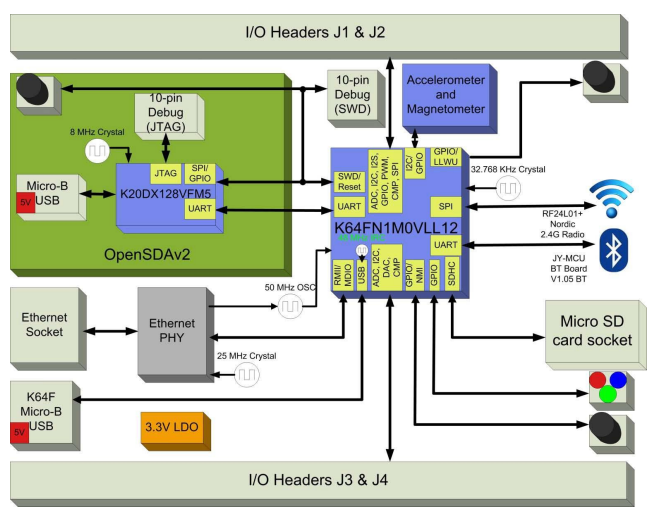
\includegraphics[width=0.9\textwidth]{diagBloquesK64F}
	\caption{Diagrama de bloques placa FRDM K64F.}\label{diagBloquesK64F}
\end{figure}

En el caso de los sistemas embebidos, cada uno de ellos se construye según el propósito específico que se va a realizar con ello, es decir, dependiendo de su objetivo tendrá unas características hardware u otras. Sin embargo, sí que hay algunos componentes mínimos presentes en todas las placas como pueden ser por ejemplo, un microcontrolador (MCU) encargado de controlar las operaciones del SE. \\
Un MCU está compuesto por un procesador, memoria RAM y ROM y puertos de entrada y salida. El MCU se encarga de ejecutar las instrucciones del programa cargado en memoria, en otras palabras, gestiona las entradas y salidas de datos. Además de este componente, necesitaríamos de más periféricos para obtener algunas funcionalidades más específicas, algunos de los periféricos que podríamos utilizar son:

\begin{itemize}
\item Sensores: humedad, temperatura, ultrasonidos, etc.
\item Actuadores: motores, leds, altavoces, etc.
\item Dispositivos de interfaz humana.
\end{itemize}


\subsection{Software}

El software embebido o empotrado reside en memoria de sólo lectura. Con relación al software y hardware utilizados en este proyecto existen 2 posibilidades de cara a cargar el programa en el microcontrolador \cite{embos}:
\begin{itemize}
\item MBED. Este es el modo en el que vienen las placas por defecto. En este modo, al conectar la placa al ordenador aparecerá como un medio extraíble y deberemos arrastrar los ficheros `.bin' en el que estaría el desarrollo de nuestro programa.
\item OpenSDA. (Open Serial and Debug Adapter) o adaptador para depuración serie y comunicación serial en castellano. OpenSDA es la interfaz de bajo costo que ofrece NXP para la depuración y programación de sus microcontroladores. En la Figura \ref{OpenSDA} encontramos su diagrama de bloques.
\end{itemize}

%\imagen{openSDA}{Diagrama de bloques de OpenSDA} \label{OpenSDA}
\begin{figure}[!h]
	\centering
	\includegraphics[width=0.6\textwidth]{openSDA}
	\caption{Diagrama de bloques de OpenSDA.}\label{OpenSDA}
\end{figure}

\clearpage

En el caso de este proyecto es necesario diferenciar algunos conceptos en lo relativo al software:

\begin{description}
\item[SO en tiempo real. \cite{SOTR} \label{ref:SOTiempoReal}] Es un sistema operativo que se utiliza para facilitar la gestión de multitareas en dispositivos con recursos y tiempos limitados \cite{SisTiempoReal}. Además, las tareas deben ser deterministas en el tiempo de ejecución. Para poder comprender adecuadamente la utilidad de un RTOS debemos conocer los siguientes conceptos:
\begin{description}
\item[Tarea.] Las tareas, a las cuales también podemos referirnos como procesos o hilos, se ejecutan de manera independiente, esto quiere decir que tienen su propio espacio de memoria. El aislamiento del espacio de memoria se garantiza mediante protección por hardware (MPU) restringiendo su acceso. Las tareas pueden tener diferentes estados según lo determine el RTOS:
	\begin{description}
		\item[Bloqueado.] La tarea está esperando un evento que puede ser un bloqueo de tipo mutex o semáforo, o una liberación de espacio en memoria .
		\item[Listo.] La tarea está lista para ejecutarse en la CPU, pero se mantiene a la espera porque la CPU ya está siendo utilizada.
		\item[En ejecución.] La tarea se está llevando a cabo.
	\end{description}
Existen distintas técnicas para la programación de estos SO:
	\begin{description}
		\item[Expropiativo.] Se ejecuta la tarea con mayor prioridad. Incluso se puede interrumpir una tarea en curso si hay otra lista con prioridad mayor. Esto tiene una mayor carga en el microcontrolador ya que tiene que gestionar el cambio de tarea.
		\item[No Expropiativo] La ejecución de la tarea es ininterrumpida y solo se detiene su ejecución si se detiene o cede el control voluntariamente.
	\end{description}
\item[Comunicación entre tareas.] Como ha ocurrido en el software realizado es común que algunas variables locales de alguna tarea deban ser utilizadas en otras tareas. Para ello existen dos opciones. La primera y más simple es la utilización de variables globales. La segunda opción es la utilización de colas y buzones que nos modifiquen o lean el valor de esa variable.
\end{description}
\item[Middelware.] Este software se encarga de `comunicar' el sistema operativo con los programas. Es un conjunto de librerías que sirven como rutinas para crear una infraestructura que ofrece servicios a los desarrolladores. Un ejemplo de \extranjerismo{middleware} seria la librería lwIP que se ha utilizado en el software del proyecto.
\item[Drivers.] Los \extranjerismo{drivers} \cite{drivers} o controladores de dispositivos proveen las instrucciones necesarias para que un dispositivo externo, por ejemplo un periférico, pueda ser controlado por el sistema operativo que el sistema embebido utilice. Dos de los \extranjerismo{drivers} más utilizados en este proyecto han sido, enet para configurar el correcto funcionamiento de la conexión en red vía cable ethernet y el \extranjerismo{driver} ADC para poder utilizar los potenciómetros.
\end{description}


\section{Tecnologías de comunicación para SE}\label{sec:Comunicaciones}

Los sistemas empotrados son capaces de comunicarse de varias formas, tanto con periféricos como entre dos o más SE. Algunas tecnologías para comunicarse entre SE serían \extranjerismo{bluetooth}, infrarrojos o wifi, entre otros. De esta manera conseguimos que podamos enviar y recibir información de otros sistemas. \\
Para la comunicación con los periféricos existen otras tecnologías acorde a sus necesidades durante el intercambio de datos. 
En los próximos dos apartados hablaremos sobre este tipo de tecnologías de comunicación y sus utilidades específicas. 

\subsection{Comunicación mediante TCP/IP}

En este apartado vamos a hablar sobre la comunicación mediante TCP/IP. \\
Se explicará cómo se lleva a cabo la comunicación en red vía cable ethernet, que es la que se ha usado en el resultado final del proyecto. Se profundizará en los protocolos que componen el modelo TCP/IP \cite{avastTcpIp} que ha sido utilizado para el establecimiento de conexión en red, envío de paquetes y cierre de la conexión en el software del proyecto. \\


\subsubsection{Modelo TCP/IP}
IBM \cite{IBMTCP} define un protocolo como ``Los protocolos son conjuntos de normas para formatos de mensaje y procedimientos que permiten a las máquinas y los programas de aplicación intercambiar información. Cada máquina implicada en la comunicación debe seguir estas normas para que el sistema principal de recepción pueda interpretar el mensaje.'' \\
Podríamos compararlo con las normas sintácticas que seguimos los humanos para hablar y entendernos los unos a los otros. En este apartado, vamos a centrarnos en el conjunto de protocolos TCP/IP que se dividen en capas o niveles. \\
La figura \ref{disposicionCapas} muestra la disposición de las capas del modelo TCP/IP.

%\imagen{protocolo-TCPIP}{Capas del modelo TCP/IP} \label{disposicionCapas}
\begin{figure}[!h]
	\centering
	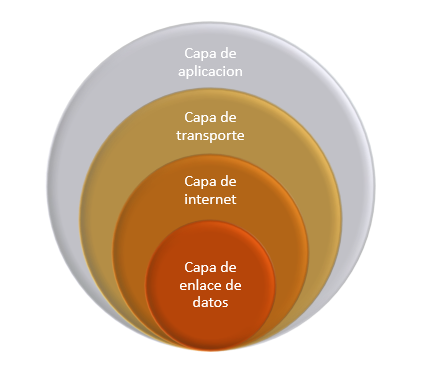
\includegraphics[width=0.9\textwidth]{protocolo-TCPIP}
	\caption{Capas del modelo TCP/IP.}\label{disposicionCapas}
\end{figure}


\begin{description}
\item[Capa de enlace de datos \cite{CapaEnlaceDatos}] 
Esta capa se encarga del intercambio de datos entre un \extranjerismo{host} y la red a la que se está conectado. Su objetivo es establecer una correcta comunicación entre las capas superiores (Red, Transporte y Aplicación) y el medio físico de transporte de datos. Esta comunicación debe ser segura entre los dos nodos, implementa un sistema de notificación de errores de la topología de la red y el control en la transmisión de las tramas. 
Esta capa se encarga de la transmisión y direccionamiento de datos sin errores y con seguridad entre nodos que pertenezcan a la misma red (comunicación punto a punto), a través del medio físico . Por otro lado, la capa de Red que es la encargada de la transmisión y direccionamiento de datos entre \extranjerismo{host} que se encuentran en redes diferentes. Ambas capas trabajan conjuntamente, puesto que la capa de Enlace de datos proporciona sus servicios a la capa de Red, ofreciendo una transmisión de datos confiable a través de un enlace físico.
Como resumen de sus principales funciones tenemos:
\begin{itemize}
\item Proporciona los servicios y medios necesarios para establecer una comunicación confiable y eficiente entre dos \extranjerismo{host}. Para ello agrega una secuencia de bits al inicio y final de los paquetes bajo un formato predefinido formando tramas.
\item Añade bits de paridad para ejercer un control de errores en el envío de las tramas. Estos bits son CRC (Códigos Cíclicos Redundantes)
\item Envía los paquetes de nodo a nodo.
\item Regula la congestión de la red.
\item Gestiona la velocidad del tráfico de datos.
\end{itemize}

\item[Capa de Internet]
La capa de Internet \cite{lopezQuesadaRED} (también denominada capa de red) controla el movimiento de los paquetes alrededor de la red. Se encarga del direccionamiento de los dispositivos y del empaquetado y manipulación de los datos para su correcto envío, entre \extranjerismo{host} que pueden estar ubicados en redes geográficamente distintas. Su misión es conseguir que los datos lleguen a su destino aunque no tengan conexión directa. Para conseguir su objetivo, ofrece servicios al nivel superior (capa de transporte) y se apoya en la capa de enlace de datos para encaminar los paquetes, mantener un control de la congestión de la red y el control de errores. 
Esta capa utiliza las versiones IPV4 e IPV6 para el encaminamiento, control y notificación de errores, existe además, IGMP (Internet Group Management Protocol) y MLD (Multicast Listener Discovery) que se usan para establecer grupos de difusión múltiple.

El protocolo IP determina el destinatario del mensaje mediante 3 elementos:
\begin{itemize}
\item Dirección IP: Dirección del equipo.
\item Máscara de subred: una máscara de subred le permite al protocolo IP establecer la parte de la dirección IP que se relaciona con la red.
\item Gateway(Puerta de enlace): le permite al protocolo de Internet saber a qué equipo enviar un datagrama, si el equipo de destino no se encuentra en la red de área local.
\end{itemize}

\item[Capa de Transporte]
La capa de transporte \cite{capaTransporte} se encarga de la segmentación de datos y ensamblaje de las partes dentro de los canales de comunicación. Esta capa se asegura de conseguir que la conexión de datos sea fiable entre dos dispositivos. Para ello, envía los datos en paquetes y se asegura de que el otro equipo indique que ha recibido los paquetes correctamente. En otras palabras, se encarga de facilitar la comunicación lógica entre dispositivos. Esta comunicación puede utilizar dos protocolos:
	\begin{description}
	\item[TCP] es un protocolo orientado a la conexión, proporciona un conjunto completo de servicios para aquellas aplicaciones que lo necesiten y su uso se considera fiable. Con el uso de puertos consigue que varias aplicaciones puedan usar una misma dirección IP. El protocolo establece una conexión virtual entre dos dispositivos capaz de enviar información de manera bidireccional. 
	\item[UDP] A diferencia de TCP, UDP no utiliza ningún mecanismo de establecimiento de la conexión, no dispone de mecanismo que aseguren, la transferencia fiable de los segmentos, por lo tanto, determinados segmentos pueden llegar a perderse. Su uso se justifica en aquellos escenarios donde la velocidad de la transmisión prima por encima de todo, aunque se incurra ocasionalmente en la pérdida de información.
	\end{description}

\item[Capa de aplicación]
Esta capa nos ofrece la posibilidad de acceder a otras capas para usar sus servicios \cite{protocolosAplicacion}. Además a esta capa, pertenecen protocolos como:
\begin{itemize}
\item Sistema de nombres de dominios (DNS): este protocolo relaciona nombres de Internet en direcciones IP.
\item Telnet: Proporciona acceso remoto a servidores y dispositivos de red.
\item Protocolo simple de transferencia de correo (SMTP): Se usa para enviar mensajes y archivos adjuntos de correo electrónico.
\item Protocolo de configuración dinámica de host (DHCP): Este protocolo asigna una dirección IP y direcciones de máscara de subred, de gateway predeterminado y de servidor DNS a un host.
\item Protocolo de transferencia de hipertexto (HTTP): Se encarga de transferir los archivos que conforman las páginas Web de la World Wide Web.
\item Protocolo de oficina de correos (POP): Es utilizado por los clientes de correo electrónico para recuperar el correo electrónico de un servidor remoto.
\item Protocolo de acceso a mensajes de Internet (IMAP): Se utiliza para recuperar correo electrónico.
\end{itemize}
Los protocolos nombrados, son usados tanto por los dispositivos de origen como de destino durante la comunicación.
\end{description}


\section{Comunicaciones para los periféricos}
Como ya mencionamos anteriormente, la mayor funcionalidad que podemos dar a estas placas viene con la condición de poder comunicarnos entre ellas y con otros periféricos. Veamos algunos tipos de conexión, además de vía ethernet o wifi, que hemos utilizado en este trabajo.

\subsection{UART}
UART, 'Universal Asynchronous Receiver-Transmitter' o en castellano Receptor-transmisor asíncrono universal. Su funcionamiento es sencillo. Utiliza solamente dos hilos para transmitir los datos. Las conexiones son cruzadas entre los dos dispositivos, es decir el pin de transmisión (TX) del dispositivo que emite el mensaje, estará conectado al pin receptor (RX) del dispositivo que recibe la comunicación y viceversa. Esta comunicación es asíncrona, por lo que no utiliza relojes para el envío y recepción de mensajes. 
Para que ambos dispositivos sepan cuando tienen que empezar y dejar leer bits se añaden a cada envío bits de inicio y parada. Es importante que ambos equipos tengan la misma tasa de Baudios configurada para que los bits se lean adecuadamente, de no ser así, la comunicación fallaría ya que un dispositivo enviaría bits a una velocidad diferente de la que se leen, ocasionando lecturas erróneas. La velocidad predeterminada suele ser de 9600 baudios. En la Figura \ref{figTramaUart} podemos ver los bits que forman una trama UART \cite{queEsUART}:

%\imagen{tramaUART}{Trama UART} \label{figTramaUart}
\begin{figure}[!h]
	\centering
	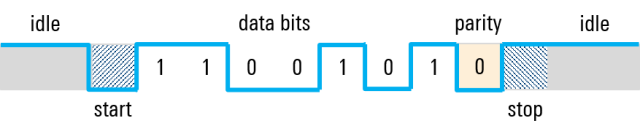
\includegraphics[width=0.9\textwidth]{tramaUART}
	\caption{Trama UART.}\label{figTramaUart}
\end{figure}

Como podemos observar los bits que forman la trama son:
\begin{itemize}
\item Bits de inicio y parada. Puesto que UART es asíncrono, son necesarios para que el receptor sepa desde dónde tiene que empezar a leer y cuando parar.
\item Bits de datos. Son la carga útil, puede haber de 5 a 9 bits por trama. 
\item Bit de paridad. Este bit se utiliza para la detección de errores en las tramas. Existen dos tipos de paridad, paridad par o impar. 
\end{itemize}

Por otro lado tenemos la comunicación USART ‘Universal Synchronous and Asynchronous Receiver-Transmitter’ que puede realizar procesos de comunicación con relojes. En la Tabla \ref{tabla:DiferenciasUART} podremos ver sus diferencias \cite{DifUartUsart} principales:

\tablaSmallSinColores{Diferencias USART y UART}{l c c}{DiferenciasUART}
{\multicolumn{1}{c}{Características} & USART & UART\\}
{
Modo & Semidúplex & Dúplex\\
Velocidad & USART es mayor & UART es menor.\\
Funcionamiento & Señales de datos y de reloj & Señales de datos\\
Datos & Bloques	& Bytes \\
Complejidad & Más complejo & Más simple de utilizar\\ 
}


El principal motivo de hacerlo con UART en vez de con USART, es su sencillez. Además los comandos de los motores se envían en bytes y no en bloques, por lo que es más directo hacerlo con UART.

\subsubsection{I2C}
El protocolo I2C, 'Inter-Integrated Circuit' usa dos líneas para comunicarse con otros dispositivos, además de las líneas de tierra y voltaje. Por un lado tenemos SCL (línea de reloj en serie) y por otro lado tenemos SDA (línea de datos), esta última es la encargada de transmitir la información. Mediante estas dos líneas el protocolo I2C es capaz de enviar datos de forma segura. Veamos algunos de los bits importantes que, tanto el maestro y esclavo \cite{hetProI2c} pueden utilizar para formar y leer las tramas:
\begin{itemize}

\item Inicio ó Start – S
\item Parada – P
\item Confirmación – ACK
\item NoConfirmación – NACK
\item Lectura-/Escritura – L/W
\item 7 bits para la dirección del dispositivo esclavo/maestro
\item 8 bits de dirección ( para algunos sensores pueden ser 16 bits)
\item 8 bits de datos
\end{itemize}
Existen distintos modos de comunicación, dependiendo de esos modos se utilizarán distinto orden y número de bits para formar las tramas. Los modos principales de comunicación son:
\begin{itemize}
\item Maestro-Transmisor y Esclavo-Receptor. Este modo se usa cuando se desea configurar un registro del esclavo I2C.
\item Maestro-Receptor y Esclavo-Transmisor. Se usa cuando queremos leer información del sensor I2C.
\end{itemize}

Este tipo de comunicación suele estar destinada al intercambio de datos con módulos o sensores y se usa en arquitecturas maestro-esclavo. Varios esclavos pueden estar conectados a un maestro al mismo tiempo pero, como es lógico, cuantos más esclavos estén conectados al maestro mayor latencia habrá en el envío y recepción de datos. Esto se debe a que solo se puede usar el bus I2C para comunicar un esclavo al mismo tiempo. También hay que tener en cuenta que dos maestros no pueden utilizar el mismo puerto. Veamos las características del maestro y el esclavo:
\begin{itemize}
\item Maestro: Dispositivo que proporciona un reloj para la comunicación. Sus funciones principales son:
\begin{enumerate}
\item Iniciar la comunicación – S
\item Enviar 7 bits de dirección – ADDR
\item Generar 1 bit de Lectura o Escritura – R/W
\item Enviar 8 bits de dirección de memoria
\item Transmitir 8 bits de datos –
\item Confirmar la recepción de datos – ACK – ACKnowledged
\item Generar confirmación de No-recepción, NACK – No-ACKnowledged
\item Finalizar la comunicación
\end{enumerate}
\item Esclavo: Dispositivo que utiliza el reloj del maestro. Sus funciones principales son:
\begin{enumerate}
\item Enviar información en paquetes de 8 bits.
\item Enviar confirmaciones de recepción, llamadas ACK.
\end{enumerate}
\end{itemize}
En nuestro caso, utilizamos este tipo de comunicación para el uso de la pantalla LCD.



\section{Periféricos}\label{sec:perifericos}
En esta parte de la memoria, vamos a ver las especificaciones de los periféricos utilizados en este proyecto

\subsection{Potenciómetro y sensor de temperatura} \label{potenySensorTemp}

El potenciómetro \cite{Potenciometro} es un elemento hardware que busca determinar un potencial eléctrico en una conexión. Generalmente, se consigue mediante la comparación de la potencia de entrada y la de salida. Esta diferencia de potencial es lo que se conoce como voltaje.
Su funcionamiento es sencillo, cuenta con tres resistencias, dos en cada uno de los extremos y una tercera resistencia con la cual podemos interactuar, permitiéndonos aumentar o disminuir su valor.

Un sensor de temperatura \cite{TempSens} es un dispositivo que transforma los cambios de temperatura (magnitud física) en señales eléctricas(voltaje). Por lo general, está  formado por un sensor encapsulado en una cubierta protectora. Entre el sensor y la cápsula encontramos un material que es  conductor térmico y que permite traspasar rápidamente estos cambios de temperatura. Existen tres tipo de sensores de temperatura descritos perfectamente en \cite{TempSensTipos}:

\begin{itemize}
\item Termopares. Funcionan mediante un principio de generación de una corriente entre dos metales diferentes unidos que tienen diferente comportamiento eléctrico en función de la temperatura. La señal generada se procesa y da lugar a una medición de temperatura. Son equipos sencillos, baratos y con una precisión suficiente para su uso en edificación. Sin embargo, tienen una respuesta lenta.
\item Termorresistencias. Están constituidas por resistencias cuya conductividad varía en función de la temperatura, lo cual genera una señal que, una vez procesada, permite obtener la medición de temperatura. Su velocidad de respuesta depende de la masa de la resistencia.
\item Sensores electrónicos. Funcionan mediante dispositivos electrónicos que generan una corriente o señal en función de la temperatura. Son equipos con una respuesta mucho más rápida, pero más caros.
\end{itemize}



\capitulo{4}{Técnicas y herramientas}

""Esta parte de la memoria tiene como objetivo presentar las técnicas metodológicas y las herramientas de desarrollo que se han utilizado para llevar a cabo el proyecto. Si se han estudiado diferentes alternativas de metodologías, herramientas, bibliotecas se puede hacer un resumen de los aspectos más destacados de cada alternativa, incluyendo comparativas entre las distintas opciones y una justificación de las elecciones realizadas. 
No se pretende que este apartado se convierta en un capítulo de un libro dedicado a cada una de las alternativas, sino comentar los aspectos más destacados de cada opción, con un repaso somero a los fundamentos esenciales y referencias bibliográficas para que el lector pueda ampliar su conocimiento sobre el tema.""

\section{Metodologias Agiles}

\section{Herramientas Hardware}

K64F
ESP8266
PLACA DE EXPANSION ARDUINO BASIC I/O

\section{Herramientas Software}

kds IDE
MCUEXPRESSO IDE
DOCKLIGTH
TERMITE

\section{Herramientas de DOCUMENTACION}
TEX
TEXMAKER
WORD

\section{Herramientas DE COMUNICACION}
EMAIL
TEAMS

\section{Herramientas de GESTION de PROYECTOS}

GITHUB
TRELLO



\capitulo{5}{Aspectos relevantes del desarrollo del proyecto}

Este apartado pretende recoger los aspectos más interesantes del desarrollo del proyecto, comentados por los autores del mismo.
Debe incluir desde la exposición del ciclo de vida utilizado, hasta los detalles de mayor relevancia de las fases de análisis, diseño e implementación.
Se busca que no sea una mera operación de copiar y pegar diagramas y extractos del código fuente, sino que realmente se justifiquen los caminos de solución que se han tomado, especialmente aquellos que no sean triviales.
Puede ser el lugar más adecuado para documentar los aspectos más interesantes del diseño y de la implementación, con un mayor hincapié en aspectos tales como el tipo de arquitectura elegido, los índices de las tablas de la base de datos, normalización y desnormalización, distribución en ficheros3, reglas de negocio dentro de las bases de datos (EDVHV GH GDWRV DFWLYDV), aspectos de desarrollo relacionados con el WWW...
Este apartado, debe convertirse en el resumen de la experiencia práctica del proyecto, y por sí mismo justifica que la memoria se convierta en un documento útil, fuente de referencia para los autores, los tutores y futuros alumnos.

\capitulo{6}{Trabajos relacionados}\label{cap:trabajosRelacionados}

Este capítulo mostrara algunos trabajos que se han hecho con sistemas empotrados. De esta manera podremos hacernos a la idea de algunas de las aplicaciones reales de estos sistemas. Veamos los distintos sectores en los que se utilizan los SE:

\section{SE en equipos médicos}\label{sec:TREquiposMedicos}

Muchos de los aparatos que se utilizan de forma periódica en la sanidad, usan un microcontrolador \cite{medicinaSE}. La Figura \ref{PresionSanguinea} muestra un ejemplo de un medidor de presión sanguínea:

%\imagen{presionSangre}{Esquema arquitectónico de un SE de medición de sangre.} \label{PresionSanguinea}
\begin{figure}[!h]
	\centering
	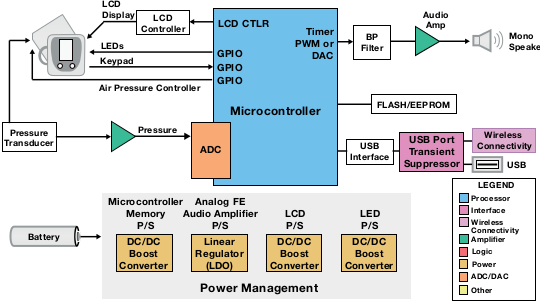
\includegraphics[width=0.9\textwidth]{presionSangre}
	\caption{Esquema arquitectónico de un SE de medición de sangre.}\label{PresionSanguinea}
\end{figure}

En la imagen podemos apreciar como existen dos partes importantes, por un lado tenemos todos los elementos que necesitan corriente y cómo se conectan a una fuente de alimentación y por otro lado está el microcontrolador al que se conectan todos los periféricos que nos ayudan a llevar a cabo la tarea que queremos realizar. Algunos de esos periféricos son un altavoz o una pantalla para poder interactuar con el usuario que use el sistema. También tenemos el sensor de presión sanguínea que utilizará un valor analógico y lo convertirá en uno digital (ADC) para poder saber la presión sanguínea del cliente.
Otro ejemplo sería la utilización de un SE para controlar un desfibrilador (DESA). Un desfibrilador sirve para recuperar el ritmo cardíaco. En la actualidad se pueden encontrar este tipo de sistema de primeros auxilios, en algunos establecimientos, generalmente en ambientes deportivos o donde el flujo de gente es de avanzada edad. Estos aparatos cuentan con un microcontrolador que mediante un altavoz explica como debes usarlo y aplica de forma cíclica una serie de descargas dependiendo del estado del paciente y con poca interacción humana. En este caso el esquema arquitectónico sería muy parecido a la figura que presentaba arriba cambiando el flujo de aire por un sensor de ritmo cardíaco. 

\section{SE en gestión de la energía}\label{sec:TRGestionEnergetica}

Todos en nuestra casa disponemos de una caldera y un termostato con el que controlamos la temperatura. Este termostato podría ser perfectamente un sistema empotrado. En este ejemplo además vamos a poder observar la importancia y utilidad de que los SE puedan comunicarse entre ellos y no solo con otros periféricos. Veamos la siguiente Figura \ref{CalefaccionSE}:

%\imagen{seCalefaccion}{Sistema de Calefaccion con SE.} \label{CalefaccionSE}
\begin{figure}[!h]
	\centering
	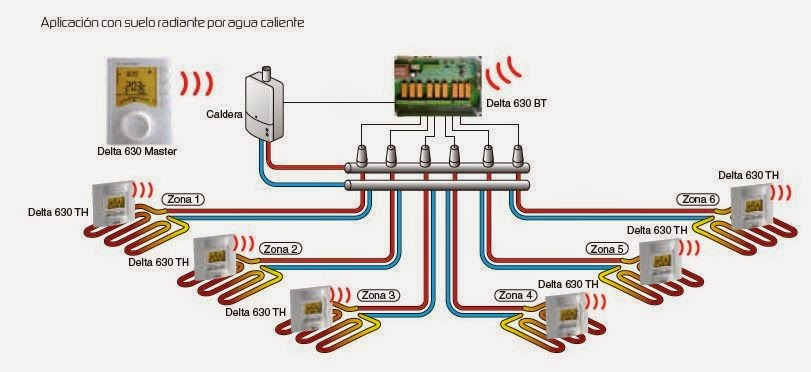
\includegraphics[width=0.9\textwidth]{seCalefaccion}
	\caption{Sistema de Calefaccion con SE.}\label{CalefaccionSE}
\end{figure}

Como podemos apreciar en la Figura \ref{CalefaccionSE} se muestran 2 sistemas embebidos, además de uno por cada zona a calentar. El primer sistema embebido, `SE1', es el que utilizará el usuario para encender la caldera y configurar la temperatura de cada zona. El SE1 se comunica con la caldera y con el `SE2'. El SE2 es el encargado de abrir o cerrar las electroválvulas que dejaran pasar el agua caliente a cada una de las zonas calentándolas. El SE2 se comunicará con cada uno de los sistemas empotrados que encontramos en cada zona para conocer la temperatura a la que están. 
Como hemos visto de esta manera podremos conseguir distintas temperaturas en cada zona dependiendo de nuestras necesidades sin necesidad de tener que subir la calefacción de todas las habitaciones de la casa o de todas las oficinas de la empresa en caso de que alguna, por ejemplo, no se esté usando en ese momento.

\section{Conexión desde otros dispositivos}\label{sec:TRConexiones}
En este apartado me gustaría hacer mención del trabajo de fin de máster que desarrolló un compañero, \cite{RPC0027}
, de esta misma universidad en el año 2018. Su TFG estaba relacionado con los sistemas empotrados. En este caso, él realizó un la conexión a Internet de una sola placa que se controlaba a través de un servidor que el gestionaba. Utilizando las interfaces propuestas en el servidor podía gestionar las luces led de la placa, tanto su color como intensidad. Me parece muy interesante la idea de poder controlar estas placas ya no solo mediante sus botones, potenciómetros, etc, sino el hecho de poder hacerlo desde un ordenador o dispositivo móvil. 
Esto es una gran idea por varias razones:
\begin{itemize}
\item En primer lugar no necesitamos de un SE que nos haga de `puente' para poder configurar las acciones de otros puesto que utilizamos un móvil u ordenador, elementos que siempre tenemos a mano. 
\item Además de esta manera conseguimos poder comunicarnos con las otras placas desde cualquier sitio y no desde donde esté físicamente ese sistema.
\end{itemize}
Roberto lo hizo, en este caso, mediante una conexión a Internet, pensando en poder comunicarnos con él aunque estemos a grandes distancias pero como se comentó en los primeros capítulos existen más formas en caso de que lo tengamos relativamente cerca, como serían bluetooth o incluso radiofrecuencias.



\capitulo{7}{Conclusiones y Líneas de trabajo futuras}

En este capítulo veremos las conclusiones llegadas tras haber terminado el proyecto. Además se expondrán algunas ideas de cómo podríamos continuar con este mismo trabajo o realizar algunos distintos también basados en los sistemas embebidos y las comunicaciones entre ellos.


\section{Conclusiones} \label{sec:Conclusiones}
En este proyecto se han trabajado conocimientos adquiridos en varias asignaturas entre las cuales destacarían:

\begin{itemize}
\item Programación concurrente y de tiempo real.
\item Administración de redes y sistemas.
\item Programación.
\item Gestión de proyectos.
\end{itemize}

Por supuesto, este trabajo también me ha hecho darme cuenta de muchos conocimientos que no tengo y he tenido que aprender.
Otra de las partes más importantes de la realización del TFG es la gestión emocional. El hecho de saber organizarte para un trabajo de tantas horas con una fecha de entrega tan lejana, junto con la realización de las demás actividades de tu vida, hacen que tengas que mejorar tus habilidades en materias como la responsabilidad, organización, fuerza de voluntad, perseverancia, entre otras, y por supuesto al mismo tiempo tienes que luchar contra otras muchos vicios contraproducente tales como la pereza y tener que sobreponerte a las adversidades. 
En cuanto a la organización y planificación del proyecto ha sido muy enriquecedor el hecho de utilizar GitHub y la metodología Scrum. De esta manera he podido ver cómo se realiza un proyecto de este tipo en un ejemplo real y aprender cómo funciona esta herramienta. Además usarla ha permitido que en caso de fallos en la programación del sistema embebido dispusiera siempre de una copia anterior que me servía como \extranjerismo{backUp}.

Dicho esto es importante hacer hincapié en que, habiendo terminado el trabajo puedo dar por completados los objetivos técnicos \ref{sec:OTecnicos}, generales \ref{sec:OGenerales} y personales \ref{sec:OPersonales}. 

Personalmente ha sido de gran interés el uso de sistemas embebidos en mi proyecto, puesto que a medida que me adentraba más en ese campo y comprendía su utilización cada vez surgían más y más usos que se le pueden dar, tal y como veremos en el próximo apartado, 'líneas de trabajo futuras'. Además su estructura permite ampliar sus funcionalidades fácilmente por lo que cada vez se utilizan más en distintos ámbitos como, industrial, electrónico, informático o incluso en la salud. 
Otra de las grandes ventajas de usar estos sistemas en la actualidad es el hecho de que se puedan comunicar entre ellas estando a pocos metros o incluso a kilómetros de distancia. 

Es de justicia decir también, que al igual que estos sistemas permiten un gran número de usos, también tienen puntos débiles. Debemos poner de manifiesto que su programación a bajo nivel puede resultar bastante complicada al principio y en muchas ocasiones se necesitan placas específicamente creadas para algunos periféricos concretos, debido a su voltaje, número de pines o funcionamiento. Esto genera que cada vez que se hace un proyecto, dependiendo de la dificultad y dimensiones de este, se deba crear un sistema específico. Además por lo general disponen de poca memoria y por lo tanto requieren que las librerías y el propio código y variables utilizadas no sean demasiado extensos, ni requieran del almacenamiento de muchos datos.


\section{Líneas de trabajo futuras}\label{sec:LTF}

Este proyecto, al tratarse de un sistema embebido, puede ser continuado en varios puntos. Las opciones son prácticamente infinitas y solo se debe imaginar un objetivo para poder continuar. Algunos puntos importantes sobre los que se podría trabajar serian:

\begin{description}
\item La integración de la conexión vía wifi con el módulo ESP8266 o semejantes. De este modo podríamos replicar el mismo proyecto u otro diferente sin depender de la utilización de cables de red. 
\item Continuando con más conexiones, también podríamos utilizar la conexión bluetooth tanto para conectar la placa o bien a un móvil o a un ordenador de modo que pudiéramos utilizar un hardware que siempre tenemos a mano para gestionar los parámetros necesarios.
\item Otra línea de futuro sería implementar algún sistema de domótica, pudiendo llegar al punto de utilizarlo en tu propia casa. Algunos ejemplos serian, continuando con la idea del sensor de temperatura conectar o bien por infrarrojos o por bluetooth un SE al aire acondicionado y que este variara la temperatura automáticamente, incluso la implementación de un sistema de reconocimiento de voz.
\item Estas placas mediante protocolos IoT y servicios como por ejemplo Azure IoT Hub permiten conectar, supervisar y administrarlos. Además se pueden conectar a la nube para subir y descargarse datos de manera que pueden crear informes sobre el funcionamiento de un sensor.
\item Relacionado con la seguridad se podría tratar de cifrar todas las comunicaciones que haya entre dispositivos mediante bluetooth o Internet. En el caso de la conexión a Internet la propia pila que se ha utilizado en este proyecto, lwIP, dispone de un tipo cifrado conocido como \extranjerismo{Transport Layer Security} (TLS) de manera que las comunicaciones entre placas estuvieran cifradas.
\item En otros ámbitos con estas placas se podría realizar proyectos para realizar una acción, como por ejemplo abrir una puerta, mediante reconocimiento biométrico, bien facial o bien dactilar.
\end{description}


% Genera la bibliografía.
\printbibliography

% Añade el aviso de la licencia.
\clearpage

\mbox{}
\vfill

\begin{figure}[!h]
  \centering
  
\includegraphics[width=0.2\textwidth]{ccbyncsa}
\end{figure}

\begin{center}
  Este obra está bajo una
  \href{https://creativecommons.org/licenses/by-nc-sa/4.0/}
    {licencia de Creative Commons Reconocimiento-NoComercial-CompartirIgual 4.0
    Internacional}.
\end{center}

\end{document}
